% This work is licensed under the Creative Commons Attribution-NonCommercial 4.0 International License.
% To view a copy of this license, visit http://creativecommons.org/licenses/by-nc/4.0/
% or send a letter to Creative Commons, PO Box 1866, Mountain View, CA 94042, USA.

% !TEX TS-program = xelatex

\documentclass[../Main/notes.tex]{subfiles}

\setcounter{chapter}{10}
\begin{document}

\chapter{Excited States}

Up until now, we have focused exclusively on methods to compute the energy and properties of molecules in their \emph{ground electronic state}.
In this chapter, we will start to discuss methods to compute electronically excited states.
We begin by discussing the nature of excited states, then we will introduce simple approaches to compute excited states, and finally we will briefly discuss more sophisticated approaches.

\section{Electronically excited states}
%In this chapter we will go over the main approaches used to compute electronically excited states.
%The problem of describing excited states is similar to that of computing ground states with pronounced static correlation effects.
%However, in many cases one can assume that the ground state is well described by a single Slater determinants or by ground state DFT, and this allows us to employ the formalism of single-reference methods as a way to build excited state methods.
%In other cases, both the ground and its excited states may display static correlation, in which case it is necessary to use a multireference method to describe both the ground and the excited states.
%This is particularly important when one is interested in computing states near a conical intersection, where two states become degenerate.
Molecular electronic excitations correspond to states in which one or more electrons are promoted (excited) from occupied to unoccupied orbitals.
Excitations from occupied valence to unoccupied valence orbitals typically fall in the UV-visible region of the spectrum and are typically referred to as \emph{valence} excitations.
It is very often the case that the lowest excited state corresponds to exciting one electron from the HOMO to the LUMO orbital.
However, molecules can undergo other type of excitations, like \emph{core to valence} excitations, which are more energetic and fall in the X-ray region of the electromagnetic spectrum.

\section{Configuration interaction singles}
Methods that target excited states specifically build approximate wave functions that contain excited determinants.
The simplest excited state method is configuration interaction with singles (CIS).
The CIS wave function is a linear combination of singly excited determinants
\begin{equation}
\Psi_\mathrm{CIS} = \sum_{i}^{\mathrm{occ}}\sum_{a}^{\mathrm{vir}} c_i^a \Phi_{i}^{a}
\end{equation}
In this equation, the notation $\Phi_{i}^{a}$ indicates a determinant obtained from the Hartree--Fock state by removing an electron from orbital $\varphi_i$ and placing it in orbital $\varphi_a$, while the quantities $c_i^a$ are coefficients associated with an excited state.
In the CIS method, the determinants are assumed to be fixed, while the coefficients $c_i^a$ are unknowns that must be determined.
Like in Hartree--Fock theory, we find the solution to this problem via minimization of the energy. Mathematically, this is equivalent to solving a matrix eigenvalue problem:
\begin{equation}
\mathbf{Hc} = E_\mathrm{CIS} \mathbf{c}
\end{equation}


\section{Time-dependent DFT}

\section{Equation-of-motion coupled cluster methods}

\section{Equation-of-motion coupled cluster theory}
\begin{equation}
\hat{H} \rightarrow \bar{H} = e^{-\hat{T}} \hat{H} e^{\hat{T}} 
\end{equation}
If 
\begin{equation}
\hat{H}  \ket{\Psi_\alpha} = E_\alpha \ket{\Psi_\alpha}
\end{equation}

\begin{equation}
\begin{split}
\hat{H}  e^{\hat{T}} e^{-\hat{T}} \ket{\Psi_\alpha} = & E_\alpha \ket{\Psi_\alpha} \\
e^{-\hat{T}} \hat{H}  e^{\hat{T}} e^{-\hat{T}} \ket{\Psi_\alpha} = & E_\alpha e^{-\hat{T}} \ket{\Psi_\alpha} \\
\bar{H} e^{-\hat{T}} \ket{\Psi_\alpha} = & E_\alpha e^{-\hat{T}} \ket{\Psi_\alpha} \\
\bar{H} \ket{\bar{\Psi}_\alpha} = & E_\alpha \ket{\bar{\Psi}_\alpha} \\
\end{split}
\end{equation}


\section{Multireference methods for excited states}




\section{CASSCF methods for excited states}
State-specific CASSCF

\begin{equation}
\ket{\Psi_\text{SS-CASSCF}^{(\alpha)}} 
= \sum_I C_I^{(\alpha)} \ket{\Phi^{(\alpha)}_I}
\end{equation}
where
\begin{equation}
\ket{\Phi^{(\alpha)}_I} =  \ket{\psi^{(\alpha)}_{i_1} \cdots \psi^{(\alpha)}_{i_N}}
\end{equation}


\begin{equation}
\ket{\Psi_\text{SA-CASSCF}^{(\alpha)}} 
= \sum_I C_I^{(\alpha)} \ket{\Phi_I}
\end{equation}

\begin{equation}
\bar{E} = \min_{C_I^{\alpha}, \{ \psi_i \}} \sum_{\alpha = 1}^{d}
w_\alpha \braket{\Psi_\text{SA-CASSCF}^{(\alpha)} | \hat{H} | \Psi_\text{SA-CASSCF}^{(\alpha)}} 
\end{equation}

%\mfigure{
%\centering{
%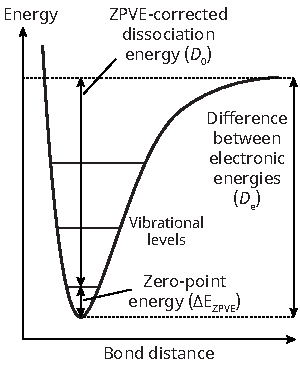
\includegraphics[width=2.00in]{img/zpve}
%}
%\captionof{figure}{Dissociation curve for a diatomic molecule. The zero-point corrected dissociation energy ($D_0$) is the difference between the energy of the dissociated molecule and the first vibrational energy level.}
%\label{fig:thermo:highaccuracy}
%}


\end{document}